
\section{RFID - Radio Frequency IDentification}
Die ursprünglich Idee war dass RFID den Barcode ablösen sollte, doch der heutige Anwendungsbereich ist bereits schon viel breiter.
Reader $\rightarrow$ Tag: Downlink \\
Tag $\rightarrow$ Reader: Uplink

\begin{tabular}[h]{c c}

\parbox{8cm}{
    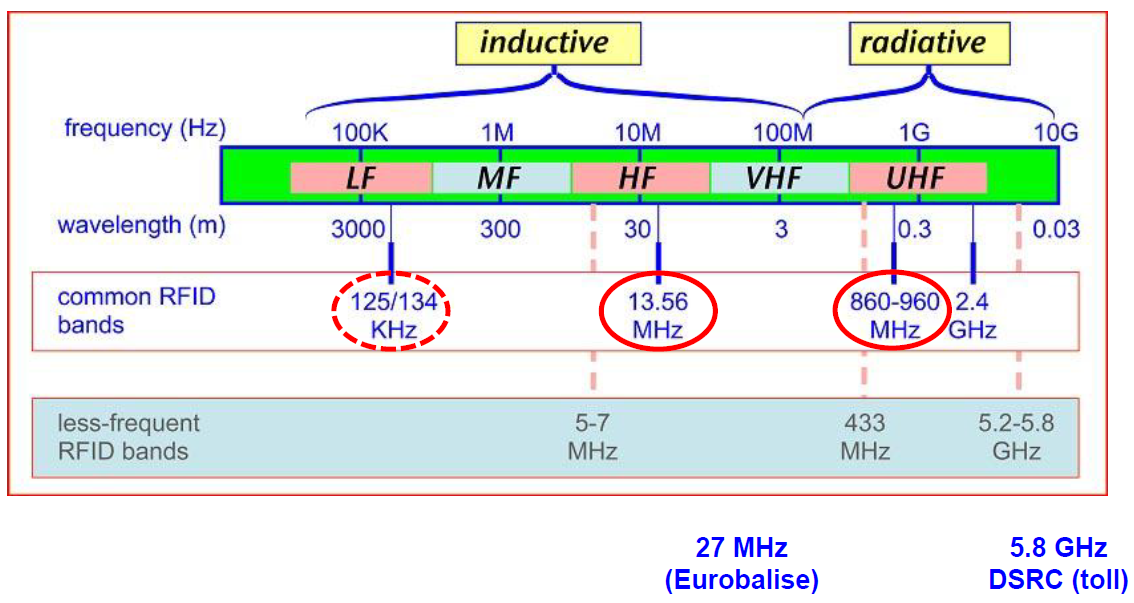
\includegraphics[width=8cm]{./bilder/RFIDFrequenzen.png} } 
&

\parbox{8cm}{
    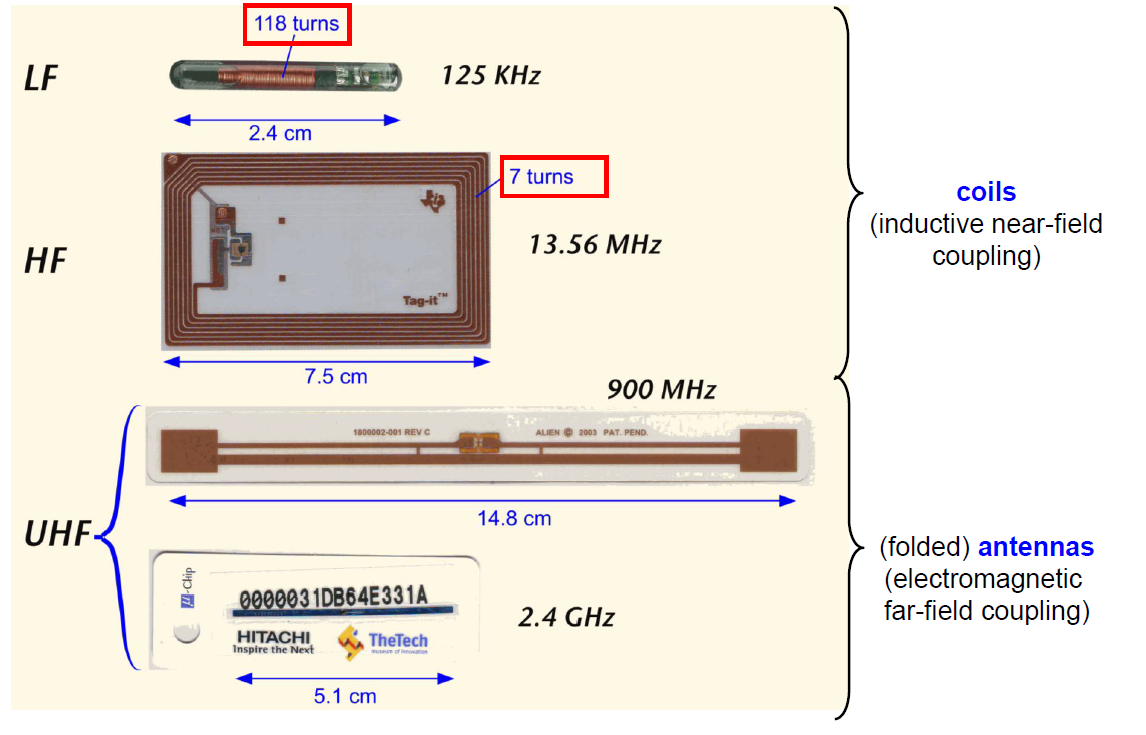
\includegraphics[width=8cm]{./bilder/RFIDTags.png} } \\
\end{tabular}
\subsection{Aktiv vs. Passiv}
	\begin{itemize}
		\item Passiv: Es sendet und empfängt gleichzeitig, Frequenzen müssen leicht verschoben sein
		\item Semi-Passiv: Es kann nur antworten, wenn es angestrahlt wird. Es hat Batterie für Tag Power aber nicht für Radioteil. 
		\item Aktiv: Es kann antworten auch wenn es nicht angestrahlt wird. Es hat Batterie für Tag und Radio. 
	\end{itemize}
\subsection{Antikollisionsprotokolle}
	\begin{tabular}{ll}
		\parbox{9cm}{
			\begin{itemize}
				 \item Deterministisches Antikollisionsprotokoll: Baumsuche anhand von uniqueID (und Maske). Leserate: 10-30 Tags/s
				 
				 \item Probabilistisches Antikollisionsprotokoll: Modifiziertes ALOHA-Protokoll (mit Random Nr). Leserate. 100-500 Tags/s
			\end{itemize}
		}	
		& \parbox{9cm}{
			\fbox{ 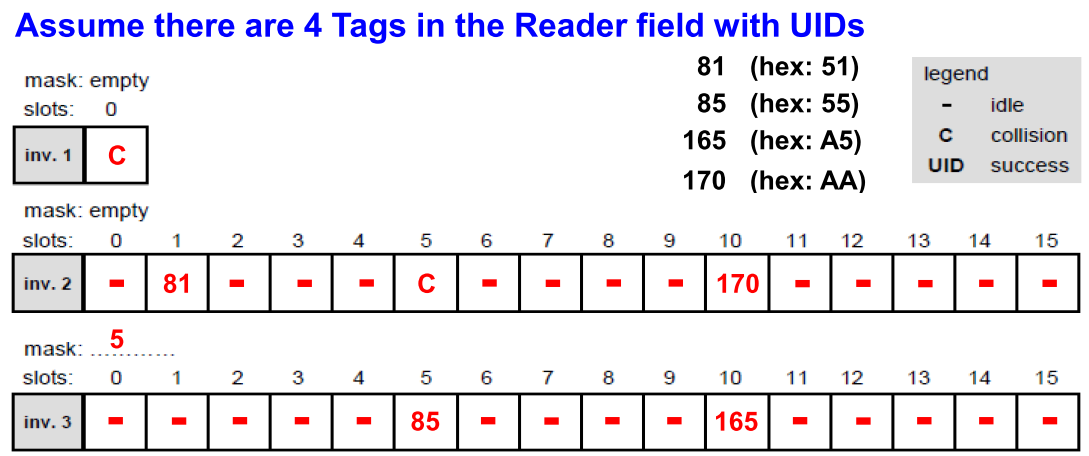
\includegraphics[width=9cm]{./bilder/rfid-anticollision.png}}\\ Bsp. Deterministic Anticollision
		}
	\end{tabular}
	
	Tags sollten einen gewissen Abstand voneinander haben um zu vermeiden dass sie sich gegenseitig stören (Schwingkreisverstimmung).

\subsection{Standards}
	\begin{itemize}
		\item LF
			\begin{itemize}
				\item ISO/IEC 11784/5 and extension 14223 identification of animals
			\end{itemize} 
		\item HF
			\begin{itemize}
				\item ISO/IEC 14443	Identification Cards – Proximity Cards (2001) 
					\begin{itemize}
						\item 2 completely different data transmission types (A and B), incompatible (Reader must support both)
						\item range up to 10 cm, data rate 106 kb/s, 13.56 MHz, inductive coupling
						\item typical application: e-ticketing, micro-payment (e.g. Metro-tickets)
					\end{itemize}
				\item ISO/IEC 15693	Identification Cards – Vicinity Cards (2001/2009)
					\begin{itemize}
						\item range up to 1m, data rate 26 kb/s, ISO/IEC 18000-3 mode 1, 13.56 MHz, inductive coupling
						\item Moving tag reading rate: 125 Tags/s (max. 1 Tag in Reader field), otherwise 10-30 Tags/s
						\item Minimum exposure time in Reader field access approx. 8 ms
						\item Deterministic anticollision-protocol (anhand von uniqueID und Maske)
						\item Memory: max. 8kByte (either 256 blocks x 256 bits or 2048 blocks x 32 bits with protocol extension)
						\item Tags are uniquely identified by a 64 bits unique identifier (UID)
						\item typical application: Access, Ski-Pass, item management
					\end{itemize}
				\item ISO/IEC 18000-3 mode 3(item management standard)
					\begin{itemize}
						\item range up to 1m, less used HF-version of EPC UHF Gen2, typically 53 kb/s (ETSI), 13.56 MHz, inductive coupling
						\item slotted ALOHA based anticollision algorithm allows up to 150 Tags/s
					\end{itemize}
						
			\end{itemize}
		\item UHF
			\begin{itemize}
				\item ISO/IEC 18000-6C item management standard - EPC (Electronic Product Code) Gen2 UHF
					\begin{itemize}
						\item Tags can be used worldwide in the 860-960 MHz band, radio coupling
						\item range up to 16m, max. ERP = 2.0 W (i.e. EIRP = 3.28 W), datarate ETSI 100kb/s (FCC: 200kb/s)
						\item slotted ALOHA based anticollision algorithm allows up to 400 Tags/s
						\item EPC is only an ID (96-496 bits), the information is stored on the network
					\end{itemize}
			\end{itemize}
		\item NFC-Interface and Protocol Standards
			\begin{itemize}
				\item NFCIP-2 (ECMA-352 / ISO-21481) 
				\item NFCIP-1 (ECMA-340 / ISO-18092) 
			\end{itemize}
	\end{itemize}	
	
\subsection{RFID LF}
	\begin{itemize}
		\item Frequenz: Um 125-134kHz
		\item Induktive Kopplung (Spulen als Empfänger) - inductive near-field coupling 
		\item Tiefe Frequenz $\rightarrow$ 100-1000 Windungen
		\item Flüssigkeiten haben nur einen geringen, Metalle haben einen grossen Störeinfluss
		\item Downlink: ASK Modulation
		\item Uplink: Load Modulation (durch kurzschliessen der Tag-Antenne wird Gegenfeld erzeugt welches Feld des Readers schwächt)
		\item Anticollision: ALOHA
		\item Typische Anwendung: Tier-Identifikation
	\end{itemize}
	
\subsection{RFID HF}
	\begin{itemize}
		\item Frequenz: 5MHz - 100MHz
		\item Typischerweise 13.56MHz (90\% aller RFID Applikationen arbeiten mit dieser Frequenz)
		\item Induktive Kopplung (Spulen als Empfänger) - inductive near-field coupling (-60dB/decade)
		\item Downlink: ASK Modulation
		\item Uplink: Load Modulation
		\item Anticollision: ALOHA
		\item Reader Talks first
		\item Hohe Frequenz $\rightarrow$ 3-10 Windungen
		\item Spulengrösse $\rightarrow$ Leseabstand = Spulendurchmesser von Reader Antenne
	\end{itemize}
\subsubsection{Modulation bei induktiver Kopplung}
	\begin{itemize}
		\item Downlink: ASK Modulation, Nicht zu viele Nullen senden, sonst hat Tag zu wenig Power. Je höher Modulationstiefe, umso weniger Energie. 
		\item Uplink: Lastmodulation, Manchester coded, Tag schliesst Antenne kurz, wird auf Hauptträger draufmoduliert (mit Subträger) $\rightarrow$
		Der Reader kann nicht auf der gleichen Frequenz ein kontinuerliches Signal senden und gleichzeitig empfangen, deshalb wir mit hilfe der Subträger
		das Spektrum verschoben (siehe Bild unten). Es kann nur 1 oder 2 Subträger verwendet werden (bei 2 Subträgerfrequenzen spricht man von FSK-Modulation).
	\end{itemize}
	
	\begin{minipage}{12cm}
		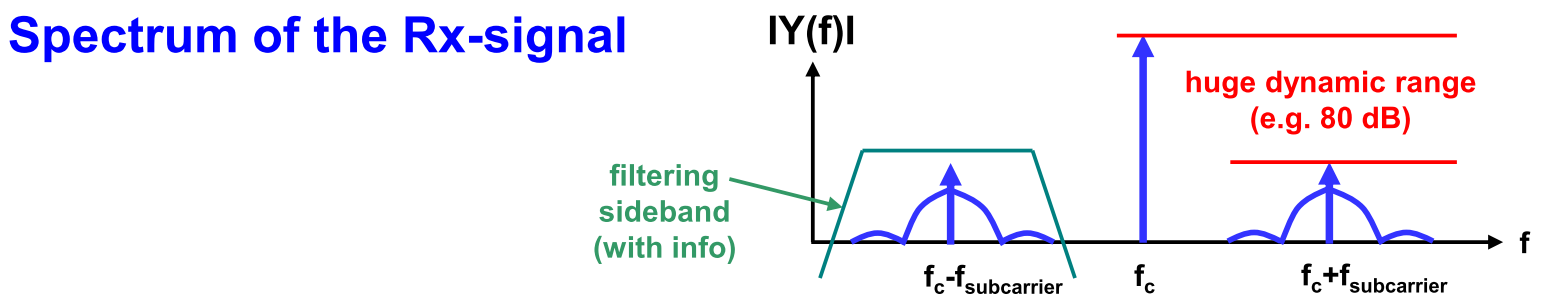
\includegraphics[width=12cm]{./bilder/rfid-spectrum.png} 
	\end{minipage}
	
	Beim Design induktiver Reader- und Tag-Antennen wird die Güte Q so gewählt, dass sich ein Kompromiss zwischen lange Distanz (hohe Spannungsspitzen) 
	und guter Träger-Subträger-Trennung ergibt.
	

\subsection{RFID UHF}
	\begin{itemize}
		\item Frequenz:	100 MHz - 10 GHz
		\item Typische Frequenzen sind 860-960 MHz oder 2.4GHz
		\item Elektromagnetische Kopplung (Antenne zum Empfangen) - electromagnetic far-field coupling
		\item Flüssigkeiten absorbieren die Strahlung und Metall hat einen grossen Einfluss
		\item Leseabstand bei passiven Tags bis zu 5-8 m (semi-passive bis 15m, aktive bis 100m)
		
	\end{itemize}

\subsubsection{Modulation bei elektromagnetischer Kopplung}
	\begin{itemize}
		\item Downlink: ASK Modulation, Nicht zu viele Nullen senden, sonst hat Tag zu wenig Power. Je höher Modulationstiefe, umso weniger Energie. 
		\item Uplink: Backscatter Modulation, Tag schliesst Antenne kurz, wird auf Hauptträger draufmoduliert (mit Miller-Modulierter Subträger)
	\end{itemize}

	\begin{minipage}{12cm}
		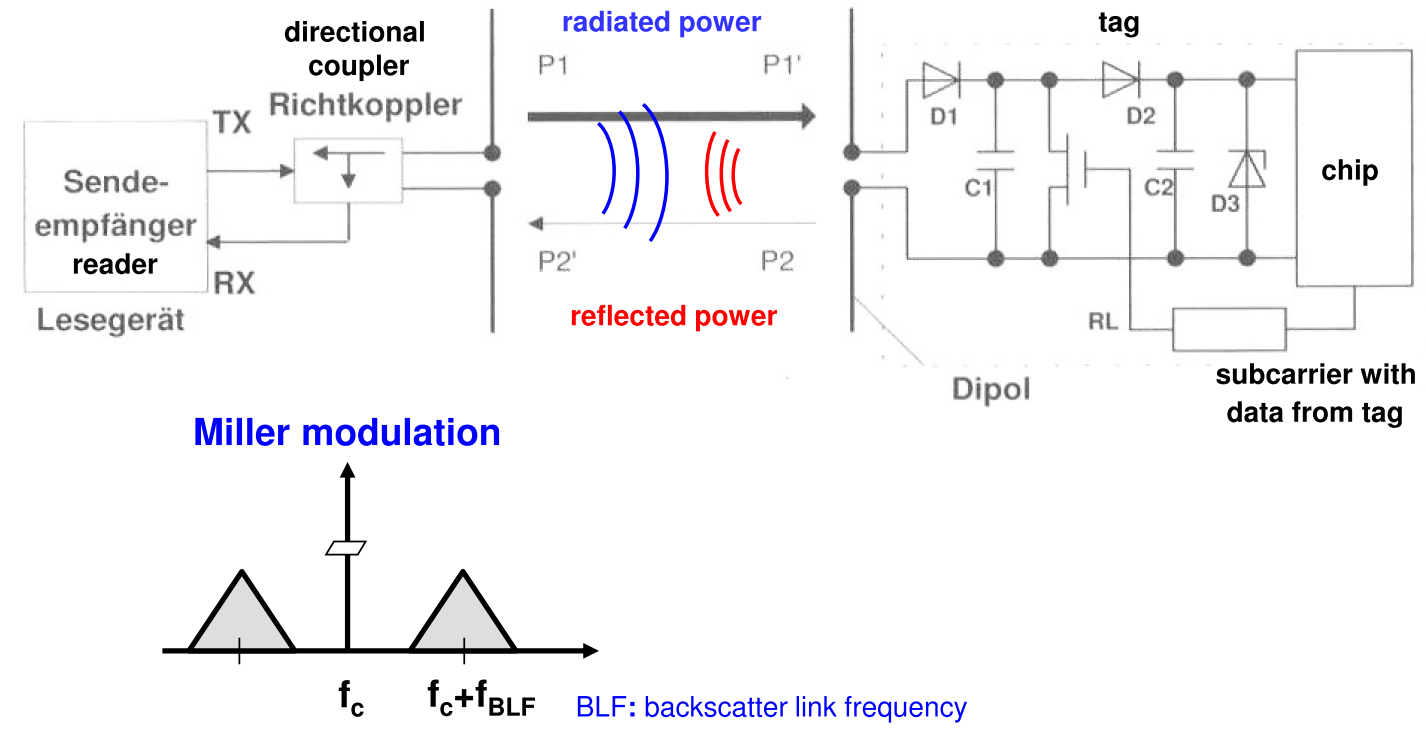
\includegraphics[width=12cm]{./bilder/rfid-millermod.png} 
	\end{minipage}
	
\subsection{NFC - Near Field Communication}
	
	\begin{minipage}{10cm}
		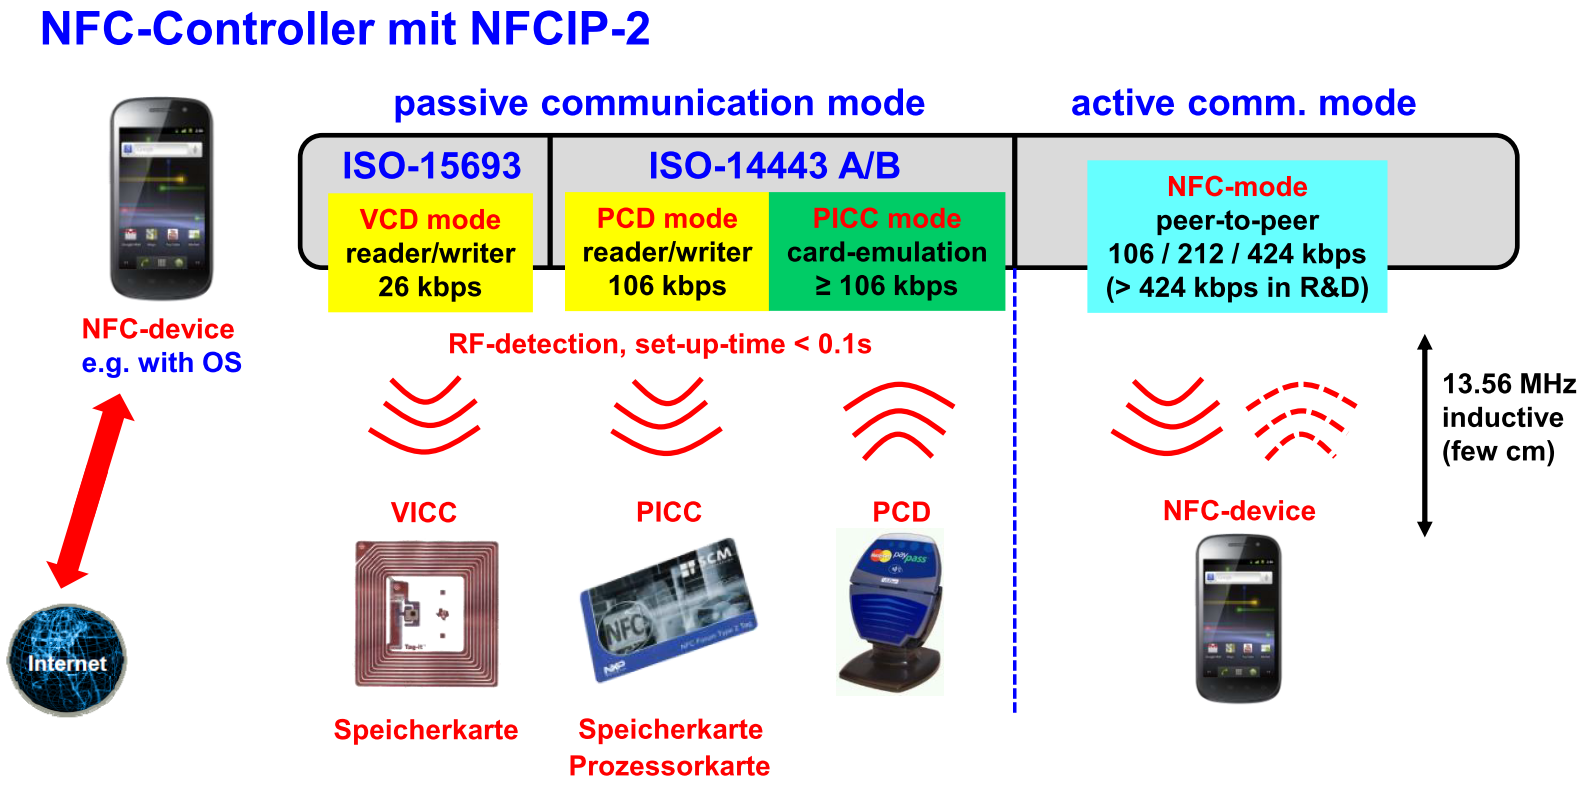
\includegraphics[width=10cm]{./bilder/rfid-nfc.png} 
	\end{minipage}
			
	NFC wird heute häufig als Synonym für RFID verwendet. NFC ist aber ein \textbf{Standard} welcher physikalisch ein RFID-Interface benutzt. 
	NFC ist beides = Auf der physikalischen Ebene RFID und auf protokol Ebene etwas Spezielles.
	\begin{itemize}
		\item Active Mode - Peer-to-Peer mode, ASK-modulation in both directions, max. 424 kb/s, range up to 20cm
		\item Passive Mode - Reader Emulation, ISO 14443 and 15693 Tags can be read
		\item Passive Mode - Card Emulation, market driver (wallet-app)
	\end{itemize}
	
	